\documentclass[12pt, a4paper, oneside, final]{article}
\usepackage[margin = 1in, bottom = 1in]{geometry}

\usepackage[T2A]{fontenc}
\usepackage[utf8]{inputenc}
\usepackage[english, russian]{babel}
\usepackage{xcolor, ulem, soulutf8, soul, fancyhdr, amsmath, amssymb, amsthm, svg, wrapfig, csvsimple, float, caption, subcaption}
\usepackage[shortlabels]{enumitem}
\usepackage{titlesec, hyperref, multicol, listings}
\usepackage[most]{tcolorbox}
\usepackage[makeroom]{cancel}
\usepackage[most]{tcolorbox}
\usepackage{tocloft, longtable, skak, stmaryrd, color}
\usepackage[framemethod = tikz]{mdframed}

\definecolor{codegreen}{rgb}{0,0.6,0}
\definecolor{codegray}{rgb}{0.5,0.5,0.5}
\definecolor{codepurple}{rgb}{0.58,0,0.82}
\definecolor{backcolour}{rgb}{0.95,0.95,0.92}
\definecolor{blueish}{rgb}{0.96,0.96,1.0}
\definecolor{grayblueish}{rgb}{0.97,0.97,0.98}
\definecolor{transblue}{rgb}{0.9,0.9,0.97}
\definecolor{transred}{rgb}{0.97,0.9,0.9}
\definecolor{light-gray}{gray}{0.95}

\renewcommand{\figurename}{}
\addto\captionsrussian{\renewcommand{\figurename}{}}
\captionsetup[table]{labelformat = empty}

\hypersetup{
	colorlinks,
	citecolor = pink,
	filecolor = pink,
	linkcolor = pink,
	urlcolor = pink
}

\lstset{
	basicstyle = \ttfamily,
	mathescape
}

\newtcblisting{mylisting}{
	listing only,
	breakable,
	colback = backcolour,
	enhanced jigsaw,
	sharp corners,
	boxrule = 0pt,
	frame hidden,
	listing options = {
		mathescape,
		commentstyle = \color{codegreen},
		keywordstyle = \color{magenta},
		numberstyle = \tiny\color{codegray},
		stringstyle = \color{codepurple},
		basicstyle = \ttfamily\footnotesize,
		breakatwhitespace = false,
		breaklines = true,
		captionpos = b,
		keepspaces = true,
		numbers = left,
		numbersep = 5pt,
		showspaces = false,
		showstringspaces = false,
		showtabs = false,
		tabsize = 4,
		inputencoding = utf8,
		language = python
	}
}

\binoppenalty = 10000
\relpenalty = 10000
\sloppy

\renewcommand*{\theenumi}{\thesection.\arabic{enumi}}
\renewcommand*{\theenumii}{\alph{enumii}}
\renewcommand*{\labelitemi}{\ensuremath{\triangleright}}

\everymath{\displaystyle}

\usepackage{tikz}
\newcommand*\circled[1]{\tikz[baseline=(char.base)]{
		\node[shape=circle,draw,inner sep=2pt] (char) {#1};}}

\begin{document}
	\thispagestyle{empty}
	\vspace*{0.5em}
	\begin{center}
		{Национальный исследовательский университет ИТМО\\Факультет информационных технологий и программирования\\Прикладная математика и информатика}\\[5.0em]
		{\Huge \bfseries Методы оптимизации}\\[0.5em]
		{\large Отчет по лабораторной работе №3}\\[0.5em]
		\textcolor{gray}{\textlangle Собрано \today\textrangle}
	\end{center}
	\begingroup
	\def\hd{\begin{tabular}{ll}
			\textbf{Работу выполнили:} \\ Бактурин Савелий Филиппович M32331 \\ Вереня Андрей Тарасович M32331 \\ Сотников Максим Владимирович M32331 \vspace*{1em} \\
			\textbf{Преподаватель:} \\ Ким Станислав Евгеньевич
		\end{tabular}
	}
	\vspace*{30em}
	\newlength{\hdwidth}
	\settowidth{\hdwidth}{\hd}
	\hfill\begin{minipage}{\hdwidth}\hd\end{minipage}
	\endgroup
	\newpage
	\section*{Решение задачи нелинейной регрессии}
	Часто решая задачу создания регрессионной модели мы сталкиваемся с тем, что по жизни очень немногие рассматриваемые функции оказываются не представимы в виде обобщенной линейной зависимости или полиномиальной некоторой конечной степени $k$.
	Такая же ситуация часто случается и с некоторым набором данных, который нужно как-то обобщить.
	Именно в таких случаях к нам на помощь приходит более частный случай регрессионного анализа~-- \textit{нелинейная регрессия}.

	Идея построения нелинейной регрессии как и в случае с полиномиальной заключается в том, чтобы найти математическую функцию, которая максимально точно описывает зависимость между независимой переменной и зависимой от нее.
	Например, для построения нелинейной регрессии можно использовать функции типа полинома, логарифмической или экспоненциальной зависимости.

	В целом весь процесс нахождения нелинейной регрессионной модели можно поделить на два этапа:
	\begin{itemize}
		\item Определить регрессионную модель $f(w, x)$, которая зависит от параметров $w = (w_{1}, ~ \ldots, ~ w_{W})$ и свободной переменной $x$.
		\item Решить задачу по нахождению минимума сумма квадратов регрессионных остатков:
		\[
			S = \sum\limits_{i = 1}^{m}{r_{i}^{2}}, ~ r_{i} = y_{i} - f(w, x_{i})
		\]
	\end{itemize}
	Однако, решая в лоб такую задачу, мы сталкиваемся с оптимизационной задачи нахождения параметров нелинейной регрессионной модели.
	Тут к нам и приходят на помощь различные методы нахождения, в том числе и рассматриваемые ниже: \textit{Gauss-Newton} и \textit{Powell Dog Leg}.
	\subsection*{Gauss-Newton}
	Напомним, что мы решаем следующую задачу: дана нелинейная модель $f(w, x)$, где $w \in \mathbb{R}^{m}$, тогда сумма квадратов регрессионных остатков высчитывается как
	\[
		S = \sum\limits_{i = 1}^{\texttt{sizeof}~X}{(f(w, x_{i}) - y_{i})^2} \to \mathrm{min}
	\]
	Итак, пусть $n = \texttt{sizeof}~X$ и введем некоторые новые объекты для решения задачи, пусть $w^{0} = (w_{0}^{0}, ~ w_{1}^{0}, ~ \ldots, ~ w^{0}_{m})$~-- начальное приближение, и
	\begin{align*}
		\gimel &= \left(\dfrac{\partial{f}}{\partial{w_{j}}}{(w^{\mathbf{i}}, x_{i})}\right)_{n \times m}~-~\text{Якобиан, или матрица первых производных} \\
		\vec{f_{\mathbf{i}}} &= \left(f(w^{\mathbf{i}}, x_{i})\right)_{n \times 1}~-~\text{вектор значений функции}~f \\
		\eth_{\mathbf{i}} &= \texttt{const}~-~\text{размера шага}
	\end{align*}
	Тогда, формула $\mathbf{i}$-й итерации рассматриваемого метода будет высчитываться как
	\[
		w^{\mathbf{i} + 1} \gets w^{\mathbf{i}} - \eth_{\mathbf{i}} \cdot \underbrace{\left(\gimel^{\mathrm{T}}_{\mathbf{i}}\gimel_{\mathbf{i}}\right)^{-1}\gimel_{\mathbf{i}}^{\mathrm{T}}}_{\beta}(\vec{f_{\mathbf{i}}} - y),
	\] где $\beta$~-- это псевдообратная матрица к матрице $\gimel_{\mathbf{i}}$, или решение некоторой задачи многомерной линейной регрессии, где мы ищем такой вектор $\beta$, что
	\[
		\left\|\gimel_{\mathbf{i}}\beta - (\vec{f_{\mathbf{i}}} - y)\right\|^{2} \to \mathrm{min},
	\] где $y$~-- вектор правильных/настоящих ответов нашей модели.
	Получается, для решения задачи, мы, так называемую, \textit{невязку} пытаемся приблизить линейной комбинацией вектора из матрицы Якобиана так, что при следующем шаге итерации получить такой $w^{\mathbf{i} + 1}$, который бы сократил нам расстояние невязки.
	Причем, заметим, что на каждом шаге, задача будет новой, так как $\gimel_{\mathbf{i}}$ зависит от текущего приближения, чтобы решить задачу многомерной регрессии.

	Заметим, что здесь, по алгоритму, мы видим достаточно очевидное ограничение: $m \geqslant n$, в ином случае для $\gimel_{\mathbf{i}}^{\mathrm{T}}\gimel_{\mathbf{i}}$ не будет существовать обратной матрицы и, в следствии, решения к уравнению.
	\subsubsection*{Исследования}
	% TODO: добавить исследования к Gauss-Newton.
	\subsection*{Powell Dog Leg}
	\textit{Trust-region method}~--- это метод решения оптимизационных задач, который основывается на вычислении региона, в котором квадратичная модель аппроксимирует целевую функцию.
	Сам этот метод представляет из себя смесь сразу двух алгоритмов, решающих задачу:
	\begin{itemize}
		\item Линейный поиск используется для определения направления поиска и дальнейшего нахождения оптимального шага вдоль выбранного вектора пути.
		\item Сам по себе trust-region используется для определения области вокруг текущей итерации, в котором модель достаточно аппроксимирует целевую функцию. Причем, стоит заметить, что для поиска следующего радиуса рассматриваемого региона также будет использоваться линейный поиск.
	\end{itemize}
	В общем случае Trust-region на каждой итерации решает следующую квадратичную задачу:
	\[
		\min_{p \in \mathbb{R}^{n}}{m_{k}(p)} = f_{k} + p^{\mathrm{T}}g_{k} + \dfrac{1}{2}p^{\mathrm{T}}B_{k}p,
	\] где $f_{k} = f(x_{k})$, $g_{k} = \nabla{f_{k}}$, $B_{k} = \nabla^{2}{f_{k}}$ и $\nabla_{k} > 0$~-- изменяющийся радиус региона, причем всё это, при условии, что $|p| \leqslant \nabla_{k}$.
	Заметим, что в таком простейшем виде мы получаем безусловно почти бесполезный алгоритм: он чрезвычайно медленный из-за появления $B_{k}$~-- Гессиана функции.
	С другой стороны, если он положительно определен и $|B_{k}^{-1}\nabla{f_{k}}| \leqslant \nabla_{k}$, то решение легко определить: $p_{k}^{B} = -B_{k}^{-1}\nabla_{k}$.
	Но, опять же, высчитывать еще и обратную матрицу~-- дело долгое и медленное, поэтому, начиная отсюда и до конца все лабораторной работы, мы будем то и дело пытаться приближать наши значения к реальным/по настоящему посчитанным значениям Гессиан-функции.

	Здесь мы рассмотрим один из методов оптимизации при аппроксимации квадратичной модели~-- \textit{Powell Dog Leg}.
	Начнем, пожалуй, с определения радиуса рассматриваемого доверительного региона: в алгоритме dogleg обычно выбирают основываясь на сходстве функции $m_{k}$ (та, что мы решаем изначально) и оригинальной функции $f$ на предыдущей итерации.
	Зададим $\rho_{k}$ следующим образом:
	\[
		\rho_{k} = \dfrac{f_{k} - f^{\star}_{k}}{m_{k}(0) - m_{k}(p_{k})},
	\] где $f^{\star}_{k} = f(x_{k} + p_{k})$.
	А теперь посмотрим на то, как именно лучше поменять шаг: в том случае, если $\rho_{k}$ меньше нуля, то это значит, что наша модель далека от функции и нужно обязательно уменьшить радиус; в том случае, изменение функции почти не изменилось и мы попали на границу региона, то есть смысл увеличить радиус; в ином другом случае~-- остается неизменным.
	\[
		\Delta_{k + 1} =
		\begin{cases}
			\dfrac{1}{4} \Delta_{k}, & \rho_{k} < \dfrac{1}{4} \\
			\min{(2\Delta_{k}, ~ \Delta_{\texttt{max}})}, & \rho_{k} > \dfrac{3}{4} \land \|p_{k}\| = \Delta_{k} \\
			\Delta_{k}, & \text{в ином другом случае}
		\end{cases}
	\]
	Наконец, начинается самое интересное со стороны Powell Dog Leg.
	Итак, мы находимся на некоторой точки нашей модели, есть подсчитанный $\Delta$-радиуса доверительного региона, и посмотрим на полный шаг $p^{B} = -B^{-1}g$.
	Если $p^{B}$ лежит в окружности региона, то мы можем его взять и более закончить алгоритм.
	В ином случае, рассмотрим анти-градиент $-g$ и попробуем вдоль нее поискать минимум квадратичной модели, то есть решить
	\[
		\min_{\|-\tau g\| \leqslant \Delta}{m(-\tau g)}
	\]
	Для её решения мы можем взять некую новую точку без каких-либо ограничений в направлении анти-градиента и найти минимум модели
	\[
		p^{U} = -\dfrac{g^{\mathrm{T}}g}{g^{\mathrm{T}}Bg}g
	\]
	Здесь снова две ситуации, где может находиться т. $p^{U}$:
	\begin{itemize}
		\item Если она находится вне рассматриваемой области, то мы можем взять точку на границе и шагнуть туда.
		\item Если же она находится в окружности, то построим отрезок $p^Up^B$ и начнем искать минимум вдоль этих двух линий $\left(\circled{\text{текущая}} \to p^U~\text{и}~p^U \to p^B\right)$.
	\end{itemize}
	Наконец, вдоль пути мы рассматриваем траекторию $\hat{p}(\tau)$
	\[
		\hat{p}(\tau) =
		\begin{cases}
			\tau p^U, & 0 \leqslant \tau \leqslant 1 \\
			p^U + (\tau - 1)(p^B - p^U), & 1 \leqslant \tau \leqslant 2
		\end{cases}
	\]
	Подытожим.
	Мы получили, на самом деле, в чем-то схожий на метод Гаусса-Ньютона алгоритм нахождения схождения, в частности, кстати, точка $p^B$~-- это то, куда бы шагнул метод Гаусса-Ньютона, но при этом, если эта точка удовлетворяет нашим потребностям, то мы действуем как Гаусс-Ньютон, в ином случае~-- чуть по другому.
	Причем под <<немного другим>> способом предполагается, на самом деле, хитрая комбинация Гаусса-Ньютона и градиентного спуска (так как при маленьком доверительном регионе мы пойдем по направлению, близкому градиентному спуску).
	\subsubsection*{Исследования}
	% TODO: добавить исследования к Powell Dog Leg.
	\newpage
	\section*{BFGS}
	\textit{BFGS}, или Алгоритм Бройдена~- Флетчера~- Гольдфарба~- Шанно~-- это тоже оптимизационный итерационный алгоритм для нахождения локального экстремума для не представимых данных или функций в линейном/полиномиальном виде.

	Один из известных квазиньютоновских методов (то есть, тех, которые основаны на получении информации о кривизне функции).
	Как и в случае с Powell Dog Leg, данный метод, в отличии от многих квазиньютоновских, использует аналог довольно медлительного постоянного переопределения Гессиана функции.
	Но если предыдущий механизм никак не взаимодействовал с явным Гессианом, то BFGS, наоборот, ускоряет работу на порядок: ибо он не явно каждый раз высчитывает матрицу, а лишь приближает к ней значения, при этом посчитав по честному Гессиан лишь один раз.

	Рассмотрим идею этого алгоритма.
	Обозначим за $x_{i} = \{x_{i}^{0}, ~ x_{i}^{1}, ~ \ldots, ~ x_{i}^{n - 1}\}$~-- координата в пространстве, где $n$~-- размерность соответствующего пространства.
	Пусть дана нам некоторая функция $f(x)$ и, как обычно, решаем задачу оптимизации нахождения $\operatorname*{argmin}_{x}{f(x)}$.
	Тогда, зададим некую начальную точку $x_{0}$ и $H_{0} = B_{0}^{-1}$~-- начальное приближение, где $B_{0}^{-1}$~-- обратный Гессиан функции, который или может быть посчитан в точке $x_{0}$, или выбран как $\mathbf{I}$~-- обратная матрица.
	Наконец, сам алгоритм:
	\begin{enumerate}[1)]
		\setcounter{enumi}{-1}
		\item Пусть $k$~-- текущий номер итерации алгоритма.
		\item Находим точку, в направлении которой будем производить поиск, она определяется следующим образом
		\[
			p_{k} = -H_{k} \times \nabla{f_{k}},
		\] где здесь и далее $f_{k} = f(x_{k})$.
		\item Вычисляем $x_{k + 1}$ через рекуррентное соотношение следующего вида:
		\[
			x_{k + 1} = x_{k} + \alpha \cdot p_{k},
		\] где $\alpha$~-- коэффициент, удовлетворяющий условиям Вольфа, которые, напомню, выглядят вот так
		\begin{align*}
			f(x_{k} + \alpha \cdot p_{k}) &\leqslant f(x_{k}) + c_{1} \cdot \alpha \cdot \nabla{f^{T}_{k}p_{k}} \\
			\nabla{f(x_{k} + \alpha \cdot p_{k})^{T}p_{k}} &\geqslant c_{2} \cdot \nabla{f^{T}_{k}p_{k}}
		\end{align*}
		\item Теперь определим размер шага алгоритма после данной итерации и изменение градиента следующими соответствующими образами
		\begin{align*}
			s_{k} &= x_{k + 1} - x_{k} \\
			y_{k} &= \nabla{f_{k + 1}} - \nabla{f_{k}}
		\end{align*}
		\item Наконец, обновим Гессиан функции, зная, что $\lambda = \dfrac{1}{y_{k}^{\mathrm{T}}s_{k}} \in \mathbb{R}$
		\[
			H_{k + 1} = \left(\mathbf{I} - \lambda s_{k}y_{k}^{\mathrm{T}}\right)H_{k}\left(\mathbf{I} - \lambda y_{i} s_{k}^{\mathrm{T}}\right) + \lambda s_{k} s_{k}^{\mathrm{T}}
		\]
	\end{enumerate}
	\subsection*{Пример}
	Возьмем в качестве примера функцию $f(x, y) = \sin{(0.5 x^2 - 0.25 y^2 + 3)} \cdot \cos{(2x+1-e^{y})}$.
	В качестве начальной точки возьмем $\langle x_{0}, y_{0} \rangle = \langle -0.3, -1.3 \rangle$ и запустим зверя.
	\begin{figure}[H]
		\centering
		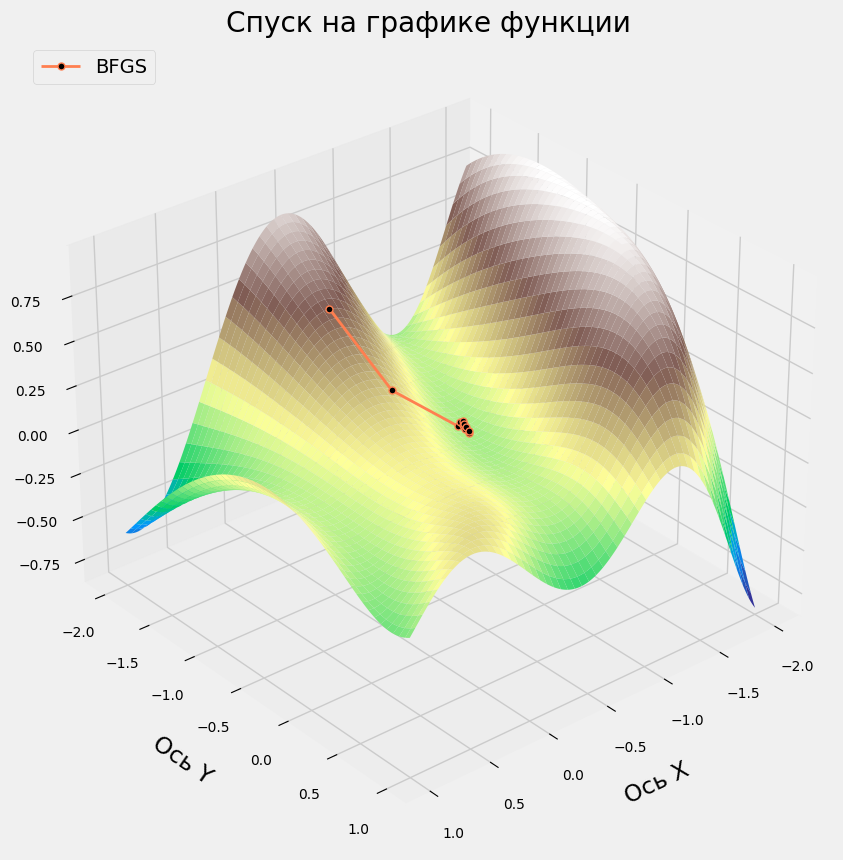
\includegraphics[scale = 0.55]{Image/T2_BFGS_3D_PLOT_1.png}
		\caption*{Example of BFGS}
	\end{figure}
	Полученные результаты столь небольшого примера с неприятным минимум следующие.
	Алгоритм сошелся к предполагаемой точке минимум за 11 шагов, после этого умер своей смертью (условие схождения).
	Полученная точка $z_{\mathtt{min}} = -0.040723$, а его прообразом служит пара из $\langle-0.848456, -0.605206\rangle$.
	Тот же путь алгоритма в виде линий уровня:
	\begin{figure}[H]
		\centering
		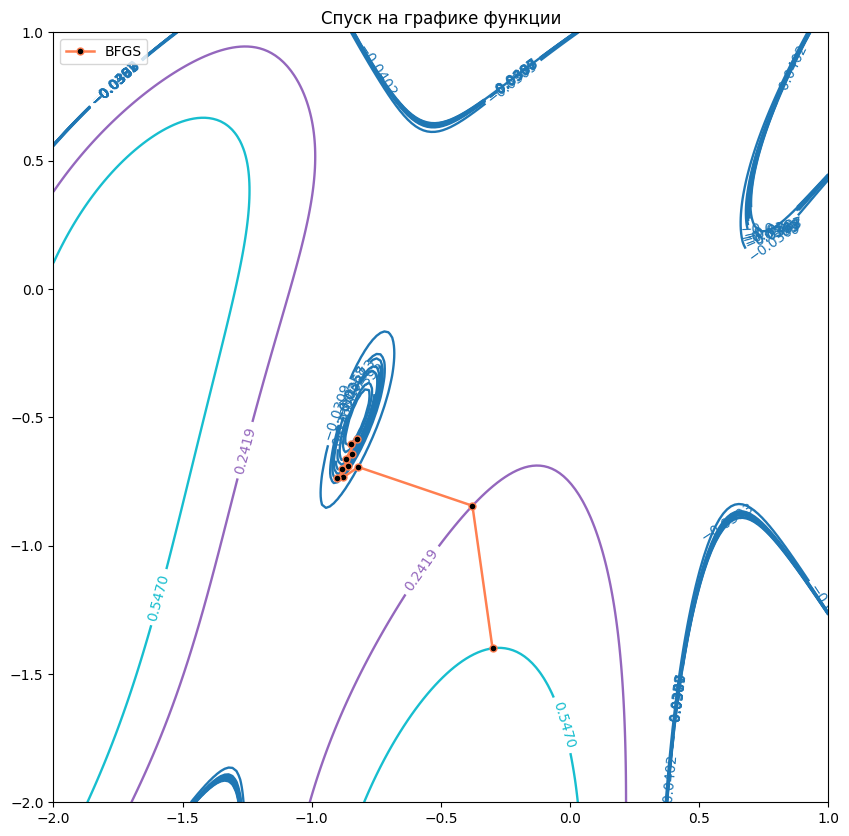
\includegraphics[scale = 0.55]{Image/T2_BFGS_LINES_1.png}
		\caption*{Example of BFGS (lines)}
	\end{figure}
	\subsection*{Исследования}
	Заметим, что исследования чистой полилинейной регрессии с методом нахождения минимальной или максимальной точки функции выглядит задачей странной, так как там нам нужен сгенерированный dataset, а здесь начальное приближение.
	Поэтому, в качестве рейтинга H(onest) за честность, мы воспользуемся BFGS как методом минимизации ошибки квадратичного уравнения.
	Его соперником выступит ранее известный нам Adam, а все-все исследования будем проводить на, внезапно, очень простой полилинейной функции $f(x) = 2 \cdot x$.
	Зададим следующие настройки генерации точек:
	\begin{align*}
		\mathtt{dots\_count} &= 500~\text{(количество точек)} \\
		\mathtt{variance}    &= 0.5~\text{(вариативность, константа, используемая в формуле генерации)} \\
		\mathtt{max\_epoch}  &= 16~\text{(максимальное количество точек)} \\
		\mathtt{batch\_min\_size} &= 0~\text{(минимальный размер батча)} \\
		\mathtt{batch\_max\_size} &= 500~\text{(максимальный размер батча)}
	\end{align*}
	Будем проводить исследования, подобно предыдущей лабораторной работы, на размере батча $\mathtt{batch\_size} \in [\mathtt{batch\_min\_size}, \mathtt{batch\_max\_size}]$.
	В качестве Adam мы возьмем результаты предыдущей лабораторной работы.
	Итак, полученный график.
	\begin{figure}[H]
		\centering
		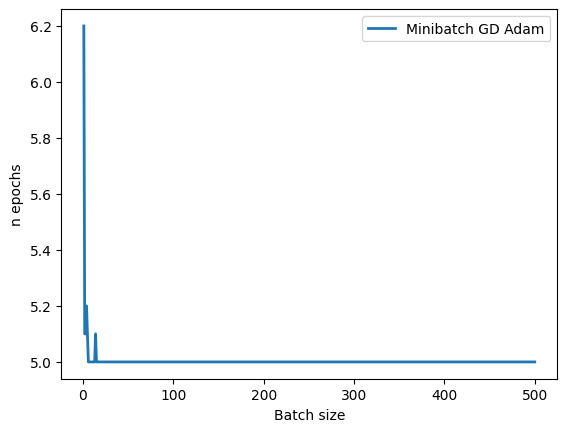
\includegraphics[scale = 0.75]{Image/T2_ADAM_GENERAL.png}
		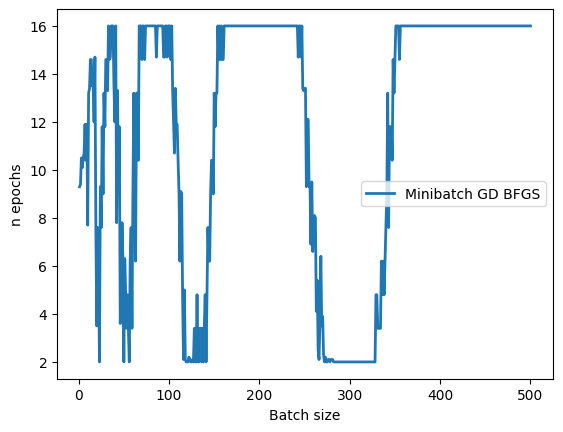
\includegraphics[scale = 0.75]{Image/T2_BFGS_GENERAL.png}
		\caption*{(Minibatch GD) Adam vs. BFGS}
	\end{figure}
	Заметим, что в большинстве случаев BFGS, по с течению обстоятельств, проигрывает великолепному Adam, у которого, по предыдущей работе, количество шагов почти никогда не изменялось и оставалось в среднем $5$.
	Также, на некоторых промежутках размеров батча BFGS всё же выигрывает гонку у Adam.
	Почему это может происходить?
	На самом деле, проблема кроется в задаче, которую мы поставили перед методами, если Adam идеален в задачах линейной регрессии, то BFGS все-таки хорош во многих нелинейных функциях (смотри пример выше).
	На примере выше мы видели, что BFGS среди множества похожих окрестностей точек минимума находит тот самый настоящий и остаётся там.

	Теперь давайте немного <<приблизимся>> к батчу $[0, 10]$ и $[0, 30]$ и посмотрим, что там происходит.
	Полученный график.
	\begin{figure}[H]
		\centering
		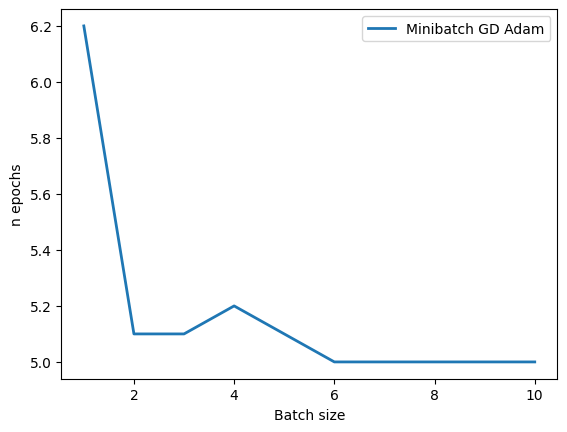
\includegraphics[scale = 0.75]{Image/T2_ADAM_1_10.png}
		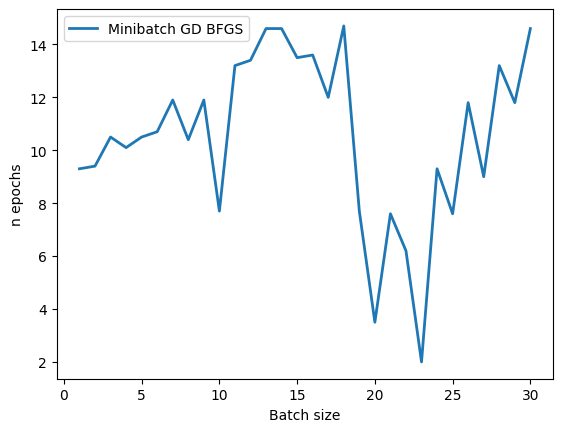
\includegraphics[scale = 0.75]{Image/T2_BFGS_1_10.png}
		\caption*{((Minibatch GD) Adam vs. BFGS) $\in [0, 10]$ и $\in [0, 30]$}
	\end{figure}
	Adam стремительно набирает скорость и падает вниз, в то время как BFGS, невооруженным взглядом заметное, что у него также скачкообразные шаги.
	При этом мы вновь видим, что при некоторых батчах также выигрывает Adam при двух или трех шагах, в отличие от пяти.

	Наконец, рассмотрим повнимательнее отрезок $[200, 500]$ у обоих методов и проанализируем.
	Получим графики.
	\begin{figure}[H]
		\centering
		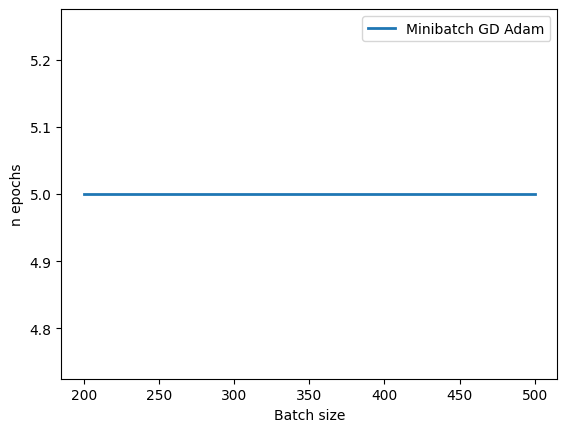
\includegraphics[scale = 0.75]{Image/T2_ADAM_200_500.png}
		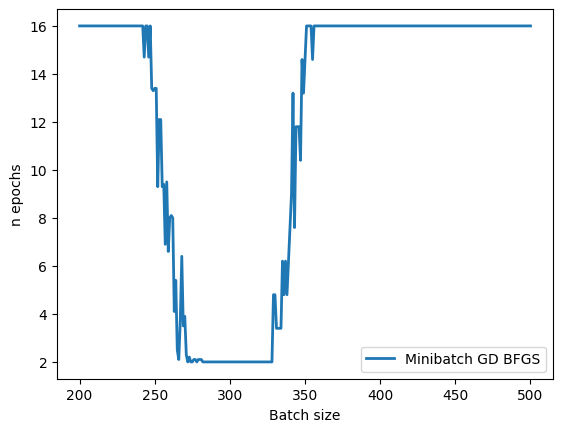
\includegraphics[scale = 0.75]{Image/T2_BFGS_200_500.png}
		\caption*{((Minibatch GD) Adam vs. BFGS) $\in [200, 500]$}
	\end{figure}
	Adam не желает перемен, в то время как BFGS пытается прогрессировать и скачкообразными шагами на промежутке от $[250 + \varepsilon, 325 + \delta]$ и доходит до минимального количества шагов.

	Подытожим результаты.
	Как мы видим, BFGS плохо справляется с минимизацией относительно столь простых функцией как прямая $f(x) = 2x$.
	Однако, в тоже время, достаточно неплохо справляется нелинейными функциями, то есть теми, которые нельзя представить как конечный полином.
	\newpage
	\section*{L-BFGS}
	\textit{L-BFGS}, или BFGS с ограниченной памятью~-- это оптимизационный алгоритм, который аппроксимирует оригинальный алгоритм BFGS с использованием заданного ограниченного объема памяти.

	L-BFGS как и BFGS использует приближенную оценку Гессиана, при этом в явном виде посчитав только один раз, а все остальные шаги лишь преобразовывая.
	Проблема: BFGS хранит всегда $n \times n$ приближений к обратному Гессиану.
	Решение: хранить несколько векторов, которые неявно представляют приближение, представляющие из себя историю последних $m$ обновлений положения $x$ и градиента $\nabla{f(x)}$.
	При этом, $m$ обычно выбирается небольшим ($m < 10$).

	Рассмотрим идею этого алгоритма.
	Во многом она будет совпадать с предыдущим, поэтому пропустим обозначения и перейдем сразу алгоритму.
	\begin{enumerate}[1)]
		\setcounter{enumi}{-1}
		\item Пусть $k$~-- текущий номер итерации алгоритма, здесь и далее будем иметь ввиду $g_{k} = \nabla{f(x_{k})}$.
		\item Также как и в BFGS находим точку, в направлении которой будем производить поиск:
		\[
			p_{k} = -H_{k} \times \nabla{f_{k}},
		\] здесь и далее $f_{k} = f(x_{k})$.
		\item Пусть мы сохранили $m$ обновлений вида:
		\begin{align*}
			s_{k} &= x_{k + 1} - x_{k} \\
			y_{k} &= g_{k + 1} - g_{k}
		\end{align*}
		Заметим, что при последующих итерациях алгоритма $k \geqslant m$ произведение из первого шага можно получить выполнив последовательность скалярных произведений и суммирования векторов, включающую $\nabla{f_{k}}$ и пары $\{s_{i}, y_{i}\}$.
		После вычисления новой итерации самая старая пара векторов в наборе пар $\{s_{i}, y_{i}\}$ заменяется новой парой, который получается из данного шага.
		\item Наконец, пожалуй, самая идейная часть~-- обновление Гессиана.
		На итерации $k$ у нас определен $x_{k}$ и пары $\{s_{i}, y_{i}\}~\forall i \in [k - m, ~ k - m + 1, ~ \ldots, ~ k - 1]$.
		Выберем некоторое начальное Гессианское приближение $H_{k}^{0}$ (в отличие от стандартной итерации BFGS, это начальное приближение может меняться от итерации к итерации) и путем повторного применения формулы, заданной изначально в BFGS, получаем
		\begin{align*}
			H_{k} &= (V_{k - 1}^{\mathrm{T}} \cdot \ldots \cdot V_{k - 1}^{\mathrm{T}}) H_{k}^{0} (V_{k - m} \cdot \ldots \cdot V_{k - 1}) \\
			&+ \rho_{k - m}(V_{k - 1}^{\mathrm{T}} \cdot \ldots \cdot V_{k - m + 1}^{\mathrm{T}})s_{k - m}s_{k - m}^{\mathrm{T}}(V_{k - m + 1} \cdot \ldots \cdot V_{k - 1}) \\
			&+ \rho_{k - m + 1}(V_{k - 1}^{\mathrm{T}} \cdot \ldots \cdot V_{k - m + 2}^{\mathrm{T}})s_{k - m + 1}s_{k - m + 1}^{\mathrm{T}}(V_{k - m + 2} \cdot \ldots \cdot V_{k - 1}) \\
			&+ \ldots \\
			&+ \rho_{k - 1}s_{k - 1}s_{k - 1}^{\mathrm{T}},
		\end{align*} где $\rho_{k} = \dfrac{1}{y^{\mathrm{T}}_{k}s_{k}}$, $V_{k} = \mathbf{I} - \rho_{k}y_{k}s_{k}^{\mathrm{T}}$.
		Из всего вышеописанного мы можем провести произведение $H_{k} \times \nabla{f_{k}}$ более эффективно следующим образом
		\begin{lstlisting}
$\alpha \gets$[0] * $\texttt{sizeof}~s$;
$q \gets \nabla{f_{k}}$;
$\forall i = k - 1, ~ k - 2, ~ \ldots, ~ k - m$ do
	$\alpha_{i} \gets \rho_{i}s_{i}^{\mathrm{T}}q$;
	$q \gets q - \alpha_{i}y_{i}$;
end
$r \gets H_{k}^{0}q$;
$\forall i = k - m, ~ k - m + 1, ~ \ldots, ~ k - 1$ do
	$\beta \gets \rho_{i}y_{i}^{\mathrm{T}}r$;
	$r \gets r + s_i(\alpha_i - \beta)$;
end
return $(-1) \cdot r \left\llbracket\equiv H_k \times \nabla{f_{k}}\right\rrbracket$;
		\end{lstlisting}
		Получение нового на данной итерации $H_{k}^{0}$ мы также сильно ускорим, лишь приблизив наши значения, используя формулу $H_{k}^{0} = \gamma_{k}\mathbf{I}$, где
		\[
			\gamma_{k} = \dfrac{s_{k - 1}^{\mathrm{T}}y_{k - 1}}{y_{k - 1}^{\mathrm{T}}y_{k - 1}}
		\]
		\item Все последующие шаги аналогичны с оригинальным BFGS.
	\end{enumerate}
	Итак, напишем идейный псевдокод алгоритма L-BFGS.
	\begin{mylisting}
function $\mathtt{is\_convergence}(f : \mathbb{R}^{n} \to \mathbb{R})$:
	/*$implementation~defined$*/

function $\mathtt{Wolfe\_coefficient}(f : \mathbb{R}^{n} \to \mathbb{R}, ~ p_{k})$:
	/*$implementation~defined$*/

function $\mathtt{get\_prod}(f : \mathbb{R}^{n} \to \mathbb{R})$:
	$\alpha \gets$[0] * $\texttt{sizeof}~s$;
	$q \gets \nabla{f_{k}}$;
	$\forall i = k - 1, ~ k - 2, ~ \ldots, ~ k - m$ do
		$\alpha_{i} \gets \rho_{i}s_{i}^{\mathrm{T}}q$;
		$q \gets q - \alpha_{i}y_{i}$;
	end
	$r \gets H_{k}^{0}q$;
	$\forall i = k - m, ~ k - m + 1, ~ \ldots, ~ k - 1$ do
		$\beta \gets \rho_{i}y_{i}^{\mathrm{T}}r$;
		$r \gets r + s_i(\alpha_i - \beta)$;
	end
	return $(-1) \cdot r \left\llbracket\equiv H_k \times \nabla{f_{k}}\right\rrbracket$;
	
function $\mathtt{LBFGS}()$:
	$x_{0} \gets \mathbf{INIT}$;
	$m \gets i \in [5, 10]$;
	$q \gets$[]
	while !$is\_convergence(f)$ do
		$H_{k}^{0} \gets \left(\dfrac{s_{k - 1}^{\mathrm{T}}y_{k - 1}}{y_{k - 1}^{\mathrm{T}}y_{k - 1}}\right)\mathbf{I}$;
		$p_{k} \gets get\_prod(f)$;
		$\alpha_{k} \gets Wolfe\_coefficient(f, ~ p_{k})$;
		$x_{k + 1} \gets x_{k} + \alpha_{k}p_{k}$
		if $k > m$ then
			q.remove($\{s_{k - m}, y_{k - m}\}$);
		$s_{k} \gets x_{k + 1} - x_{k}$;
		$y_{k} \gets \nabla{f_{k + 1}} - \nabla{f_{k}}$;
		q.append($\{x_{k}, y_{k}\}$);
	\end{mylisting}
	\subsection*{Пример}
	Возьмем в качестве примера функцию Растригина, описываемая как $f(\vec{x}) = 10n + \sum\limits_{i = 1}^{n}{\left(x_{i}^{2} - 10 \cdot \cos{(2 \cdot \pi \cdot x_{i})}\right)}$, где $-5.12 \leqslant x_{i} \leqslant 5.12$, $n$~-- исследуемая размерность.
	Здесь глобальный минимум $f(0, \ldots, 0) = 0$.
	В качестве начальной точки возьмем далеко от минимума и запустим зверя.
	\begin{figure}[H]
		\centering
		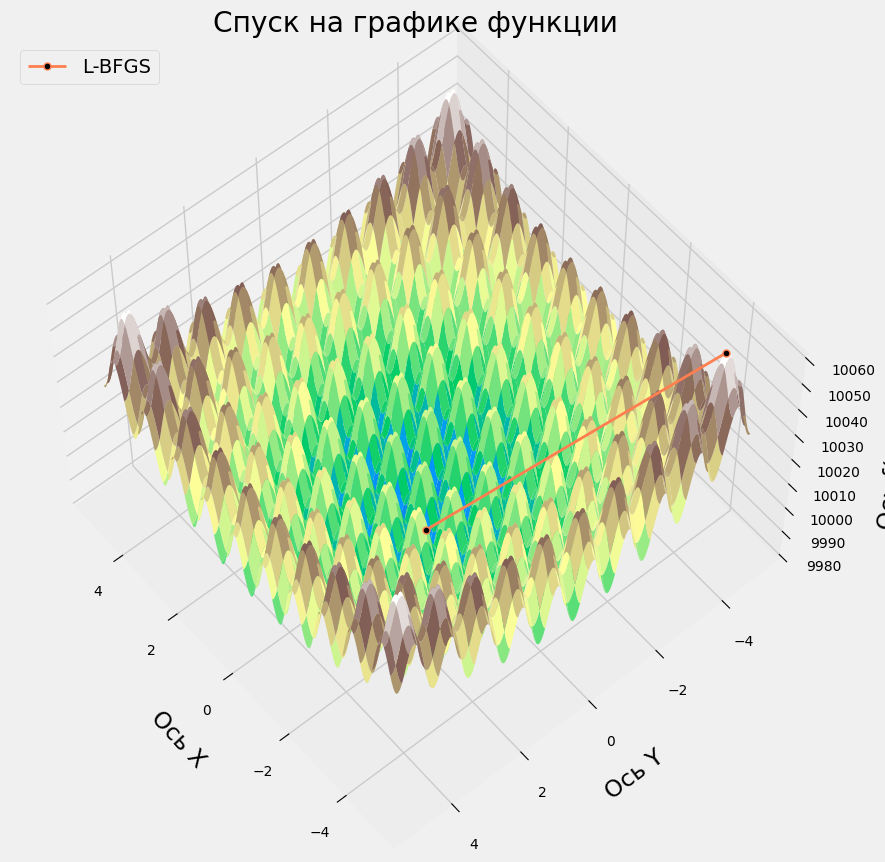
\includegraphics[scale = 0.55]{Image/AT1_LBFGS_3D_PLOT_1.png}
		\caption*{Example of L-BFGS}
	\end{figure}
	--- "Туда нам надо",~-- сказал L-BFGS и сделал один длинный шаг ровно в минимум.
	Полученная точка примерно такая же, что и заявленный минимум.
	\subsection*{Исследования}
	В качестве исследования здесь мы проведем аналогичные как и в BFGS.
	То есть, та же функция $f(x) = 2x$, и Adam как метод минимизации для линейной регрессии.
	Итак, зададим те же настройки и получим полный график по батчам $[0, 500]$.
	\begin{figure}[H]
		\centering
		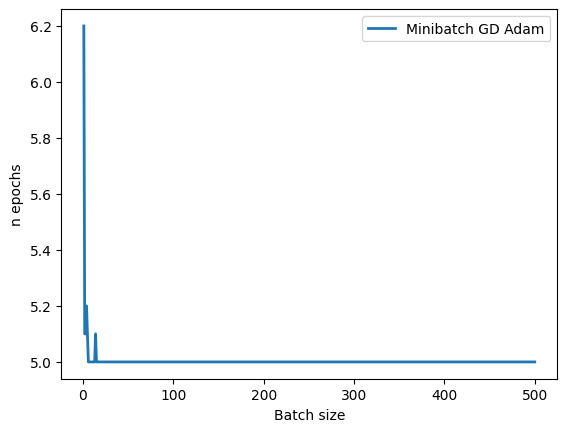
\includegraphics[scale = 0.75]{Image/T2_ADAM_GENERAL.png}
		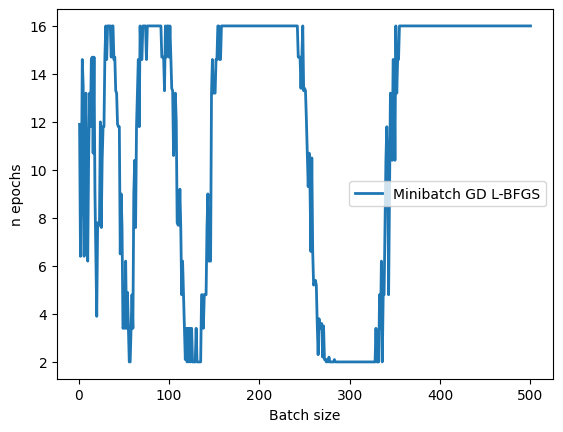
\includegraphics[scale = 0.75]{Image/AT_LBFGS_GENERAL.png}
		\caption*{(Minibatch GD) Adam vs. L-BFGS}
	\end{figure}
	Получаем аналогичные результаты, что и предыдущий пациент.
	Связано это с тем, что там и здесь используется одна и та же идея, и, по сути, разница лишь в использовании памяти, которую BFGS жрет как не в себя.
	Аналогично рассмотрим наши результаты поближе на отрезке $[200, 500]$:
	\begin{figure}[H]
		\centering
		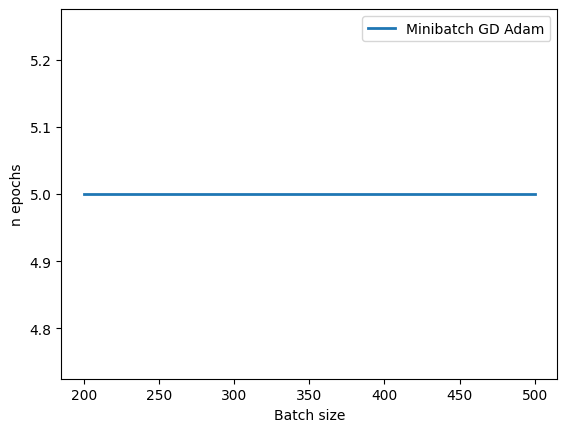
\includegraphics[scale = 0.75]{Image/T2_ADAM_200_500.png}
		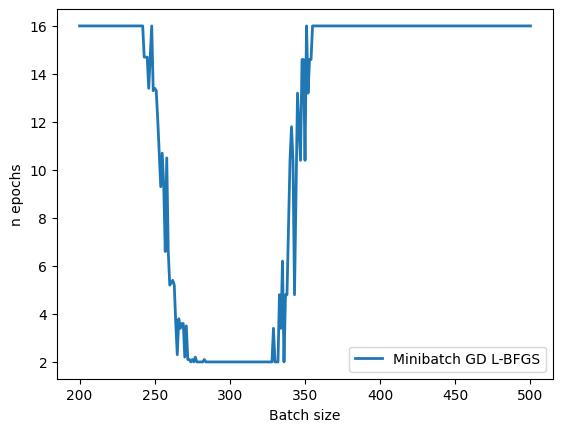
\includegraphics[scale = 0.75]{Image/AT_LBFGS_200_500.png}
		\caption*{((Minibatch GD) Adam vs. L-BFGS) $\in [200, 500]$}
	\end{figure}
	И, наконец, приближении в отрезок $[0, 10]$ и $[0, 30]$ в случае с LBFGS:
	\begin{figure}[H]
		\centering
		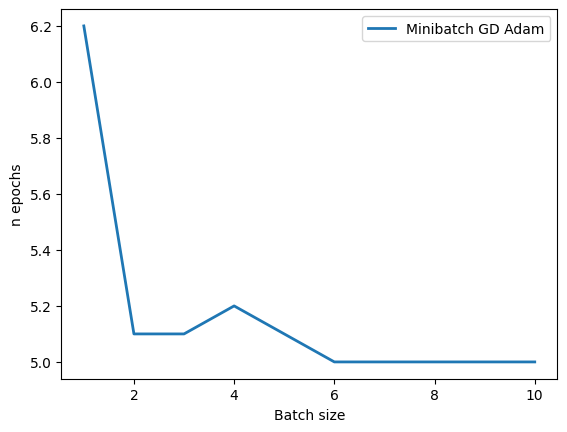
\includegraphics[scale = 0.75]{Image/T2_ADAM_1_10.png}
		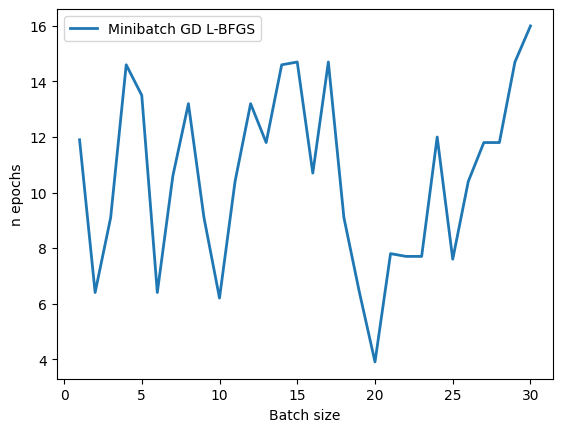
\includegraphics[scale = 0.75]{Image/AT_LBFGS_0_30.png}
		\caption*{((Minibatch GD) Adam vs. L-BFGS) $\in [0, 10]$ и $\in [0, 30]$}
	\end{figure}
\end{document}
